\documentclass[12pt]{article}
 
\usepackage[margin=1in]{geometry} 
\usepackage{amsmath,amsthm,amssymb}
\usepackage{hyperref}
\usepackage{graphicx}
\usepackage{xcolor}
\usepackage[many]{tcolorbox}
\tcbuselibrary{listings}
\usepackage{listings}
%jari:
\usepackage{enumitem}

\definecolor{lg}{HTML}{f0f0f0}

\newtcblisting{pycode}{
    colback=lg,
    boxrule=0pt,
    arc=0pt,
    outer arc=0pt,
    top=0pt,
    bottom=0pt,
    colframe=white,
    listing only,
    left=15.5pt,
    enhanced,
    listing options={
        basicstyle=\small\ttfamily,
        keywordstyle=\color{blue},
        language=Python,
        showstringspaces=false,
        tabsize=2,
        numbers=left,
        breaklines=true
    },
    overlay={
        \fill[gray!30]
        ([xshift=-3pt]frame.south west)
        rectangle
        ([xshift=11.5pt]frame.north west);
    }
}

\lstset{
    language=Python,
    basicstyle=\small\ttfamily,
}

 
\begin{document}
 
\title{Exercise 5}
\author{Jari Mattila - 35260T\\
ELEC-E8125 - Reinforcement Learning}

\maketitle

\section{Task 1}

Implement policy gradient for the CartPole environment with continuous
action space. Use agent.py for implementing the reinforcement learning algorithm itself (for
example, the agent and policy classes). Use these classes to implement the main training loop
in the cartpole.py file, similarly to how it was done in Exercise 1.
\newline

Use constant variance $\sigma^2 = 25$ for the output action distribution throughout the training.

%\begin{itemize}
\begin{enumerate}[label=(\alph*)]
    \item basic REINFORCE without baseline, 
   
The training performance plots for each of the tasks (Task 1a, b and c, Task 2 - for
different sigma values)
\newline

sgdhdjyfjghjfgjfghjf

    \item REINFORCE with a constant baseline $b = 20$,

The training performance plots for each of the tasks (Task 1a, b and c, Task 2 - for
different sigma values)
\newline

fgfhdhjfhjfgh
    
    \item REINFORCE with discounted rewards normalized to zero mean and unit variance

The training performance plots for each of the tasks (Task 1a, b and c, Task 2 - for
different sigma values)
\newline

rgdthdhgfdghdfhggf 

\end{enumerate}
%\end{itemize}

using Figure.~\ref*{fig:fig1}


\begin{figure}[h] 
	\centering  % Remember to centre the figure
    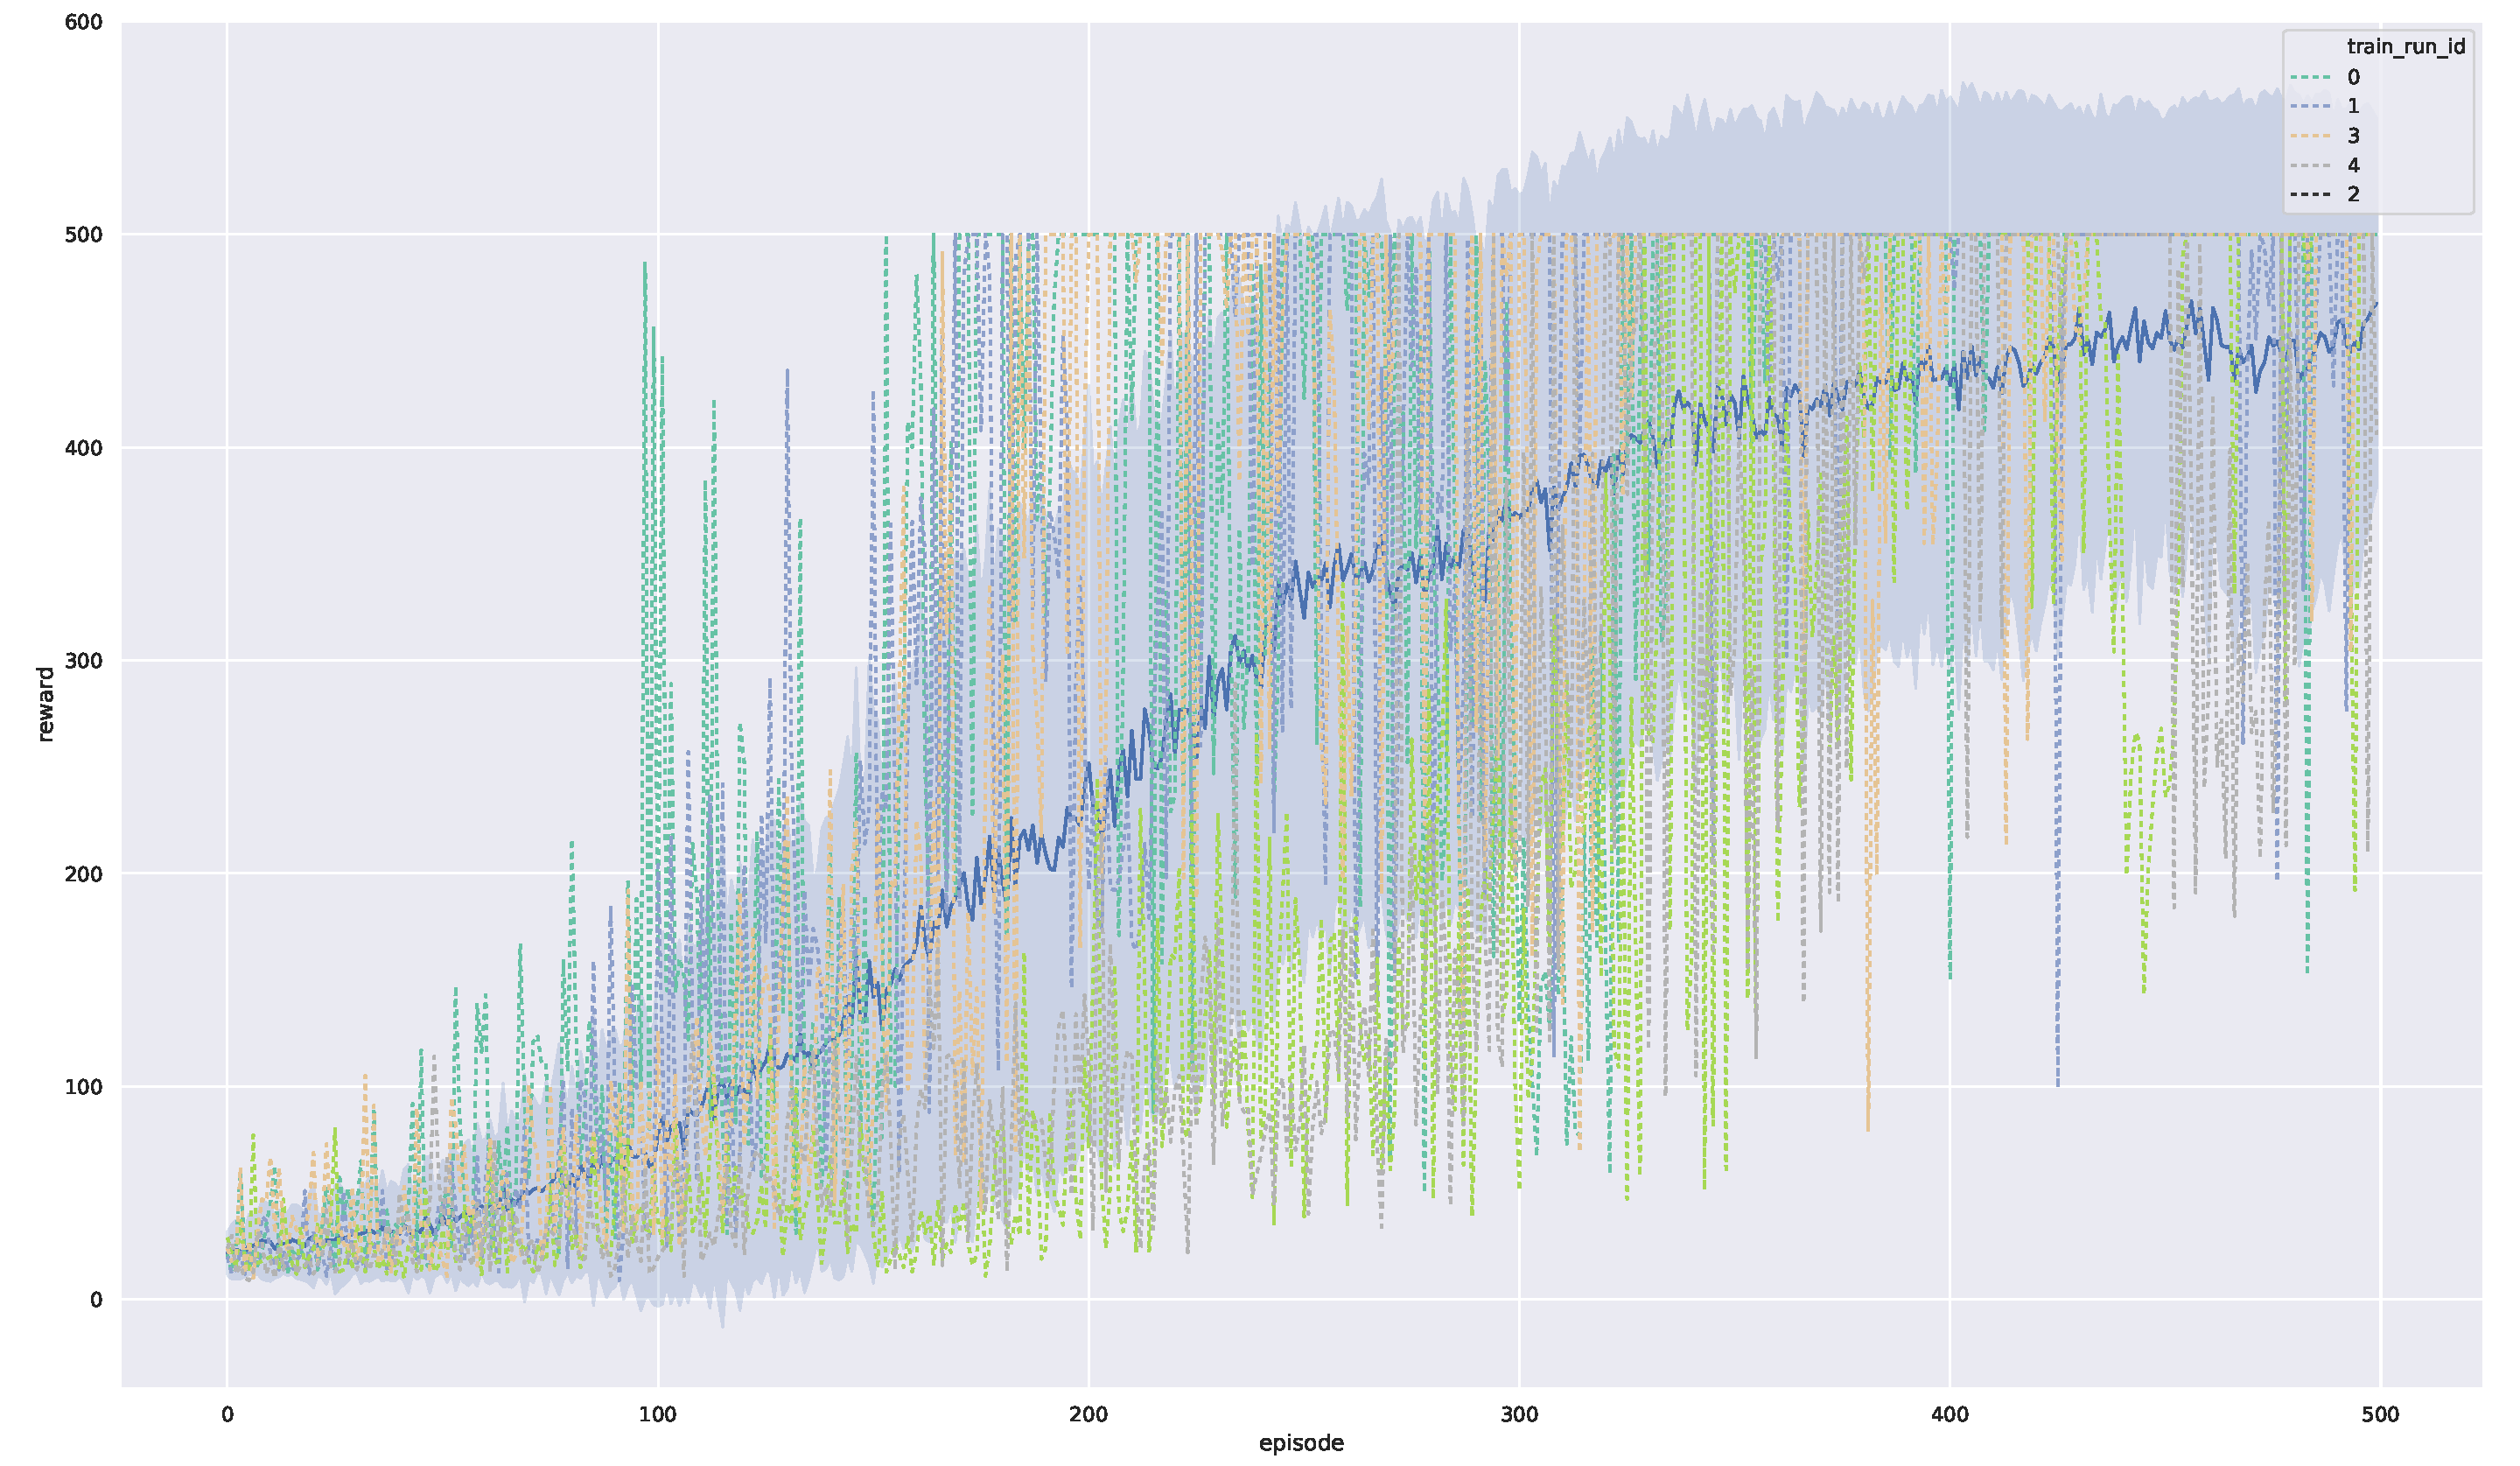
\includegraphics[width=0.9\columnwidth]{img/training.pdf}
	\caption{This is a sample figure.}
	\label{fig:fig1}
\end{figure}



\section*{Question 1.1}

How would you choose a good value for the baseline? textbf{Justify your
answer.}

\section*{Question 1.2}

How does the baseline affect the training, and textbf{why?}


\section{Task 2}

Implement two cases of adjusting variance during training: exponentially
decaying variance $\sigma^2 = \sigma_0^2 \cdot \operatorname{e}^{-c \cdot k}$
(where $c = 5 \cdot 10^{−4}$ and $k$ is the number of episode) and variance
learned as a parameter of the network (in both cases set the initial value $\sigma_0^2$ 
to 100). Use REINFORCE with normalized discounted returns for this task. The expected results for the learned variance case are shown in Figure 1.
\newline

The training performance plots for each of the tasks (Task 1a, b and c, 
Task 2 - for different sigma values)

\section*{Question 3.1}

Compare using a constant variance, as in Task 1, to using exponentially decaying variance and to learning variance during training. \textbf{Please explain} what the strong and weak sides of each of those approaches are.

\section*{Question 3.2}

In case of learned variance, what’s the impact of initialization on the
training performance? \textbf{Please explain.}

\section*{Question 4.1}

Could the method implemented in this exercise be \textbf{directly} used
with experience replay? \textbf{Why/why not?}

\section*{Question 4.2}

Which steps of the algorithm would be problematic to perform with
experience replay, if any? \textbf{Explain your answer.}


\section*{Question 5.1}

What could go wrong when a model with an unbounded continuous
action space and a reward function like the one used here (+1 for survival) were to be used with
a physical system?


\section*{Question 5.2}

How could the problems appearing in Question 5.1 be mitigated
without putting a hard limit on the actions? \textbf{Explain your answer.}

\section*{Question 6}

Can policy gradient methods be used with discrete action spaces?
Why/why not? Which steps of the algorithm would be problematic to perform, 
if any? \textbf{Explain your answer.}
















\bibliographystyle{ieeetr}
\bibliography{template}  % Modify template with your bibliography name
\end{document}
